\section{Machine Learning}
\label{sec:ml_body}
\emph{In short: classifiers trained on weak labels from the mass spectrum reach a test AUC of $0.86$; a cut on their score leaves $\Araw$ unchanged, and an adaptive partition of the Dalitz plane shows the pattern of the fixed binning.}
The mass fits separate signal from background through the shape of the mass spectrum. As a complementary, data-driven approach, classifiers were trained to separate them from the other variables of the candidates, and used to test whether a machine-learning selection changes $\Araw$ and to partition the Dalitz plane without fixing the binning in advance.
\subsection{Weak Labels and Classifiers}
\label{sec:ml_labels_body}
\label{sec:ml_models_body}
No candidate carries a true label, so the classifiers were trained on weak labels derived from the mass spectrum (\emph{weak labels}), following the classification-without-labels approach~\cite{cwola}: a classifier that separates two mixtures with different signal fractions, here the window $|m-\mu|<2\sigma$ ($15{,}130$ signal-like candidates) and the sidebands $[5150,\mu-4\sigma]\cup[\mu+4\sigma,5600]\,\MeV$ ($1940$ background-like), is, by the Neyman-Pearson lemma, also the optimal signal/background classifier (it is monotonic in the signal-to-background ratio), provided that the features carry no information on the mass. The $20$ features are the kinematic and particle-identification variables of the three tracks and two vertex variables of the $B$; the mass is not an input. Figure~\ref{fig:ml_labels} shows the regions on the mass spectrum. The classes are imbalanced ($0.128$) and are balanced with class weights, and the sample is split $60/20/20$ into training, validation and test sets. Six classifiers were compared: logistic regression with $L2$ and $L1$ penalty, a decision tree, a Random Forest, gradient boosting and a feed-forward neural network (FFNN). The tree ensembles and the network reach a test AUC of $0.857$--$0.864$, $0.09$ above the linear models and $0.04$ above the single tree, and are indistinguishable from each other within the uncertainty of the test set ($0.012$); gradient boosting, the best in cross-validation, is the reference.

\begin{figure}[h]
\centering
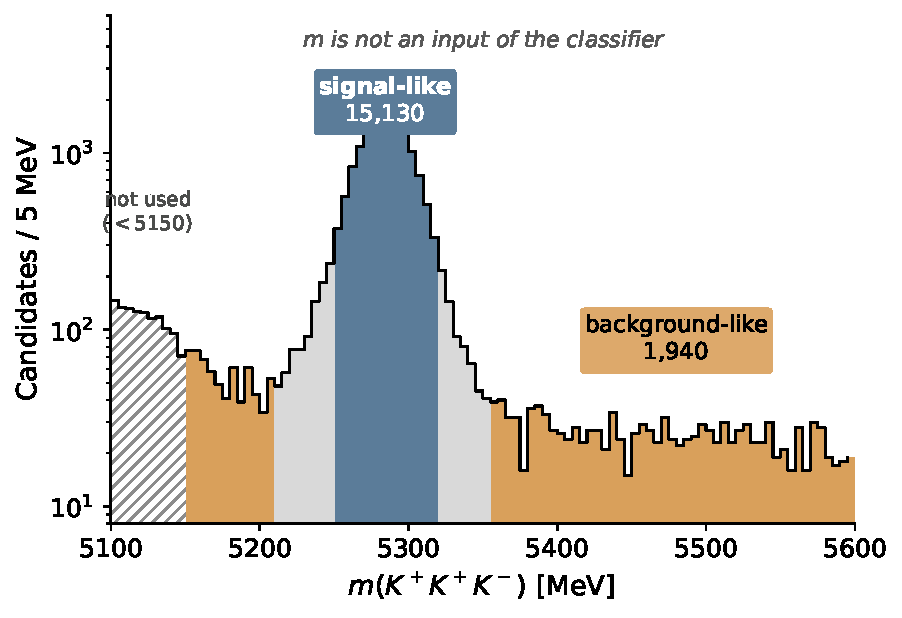
\includegraphics[width=\columnwidth]{figures/short_ml_labels.pdf}
\caption{Weak labels on the mass spectrum of the fit window: signal-like candidates ($|m-\mu|<2\sigma$, $15{,}130$) and background-like candidates (sidebands beyond $4\sigma$ and above $5150\,\MeV$, $1940$); the $2$--$4\sigma$ gap is left unlabeled and the region below $5150\,\MeV$, where the background rises towards partially reconstructed decays, is excluded.}
\label{fig:ml_labels}
\end{figure}

\subsection{Regularization, Bias-Variance and Uncertainty}
\label{sec:ml_regcal_body}
\label{sec:ml_uncertainty_body}
The regularization strength of the logistic regression, scanned over $30$ values of $C=1/\alpha$ with cross-validation, gives the same optimal AUC for the $L1$ and $L2$ penalties ($0.7686$) and no overfitting: the limitation of the linear model is its decision boundary, not the variance. For gradient boosting, whose complexity grows with the number of stages, the test AUC rises up to $\sim150$ stages and then stays at $0.865$ while the training AUC keeps rising (the gap grows from $0.018$ at $20$ stages to $0.084$ at $300$): the additional stages overfit without gain. %Class weights bias the probabilities, which converge to $\tilde p=w_sp/[w_sp+w_b(1-p)]$ instead of $p$; an isotonic recalibration on held-out folds corrects it without changing the ranking.
The uncertainty of a prediction was estimated from the spread of the $300$ trees of the Random Forest, of $300$ forward passes with dropout kept active (MC dropout) and of a deep ensemble of $10$ networks: the mean per-candidate values are $0.178$, $0.095$ and $0.050$; they measure different sources of variability, and only the Random Forest spread decreases visibly with the size of the training set ($0.220$, $0.204$, $0.179$ with a quarter, half and all of it), the epistemic part, while the part at scores around $0.5$ is the aleatoric one.
\subsection{Effect on the Measurement and Dalitz Partition}
\label{sec:ml_stability_body}
\label{sec:ml_kmeans_body}
A cut at $0.5$ on the score keeps $92\%$ of the fitted signal and $36\%$ of the background ($15{,}709$ candidates). The raw asymmetry is \textbf{stable} (Fig.~\ref{fig:ml_three}): $-0.0451\pm0.0087$ (Bayesian) and $-0.0447\pm0.0086$ (Frequentist), against $-0.0443$ and $-0.0441$ for the full window, all shifts within the spread expected for a subsample and $5.2\sigma$ from zero in both samples. The precision does not improve, because the nominal sample has little background to remove ($\approx4\%$ in the signal window). The mass spectrum, instead, changes ($\chi^2$ from $164/88$ to $253/88$ in the Bayesian fit): the classifier does not sculpt the mass, since without the nine momentum components the degradation is the same ($\chi^2=533/388$ in the Frequentist fit), but the selection changes the composition of the background, keeping partially reconstructed decays that the model does not describe. Finally, $K$-means with $K=8$ on $(m^2_{\mathrm{lo}},m^2_{\mathrm{hi}})$, an \emph{unsupervised} partition learned from the density of the candidates and stable between initializations, finds two clusters beyond $3\sigma$ ($\chi^2=46.4$ for $7$ degrees of freedom) with the pattern of the fixed binning ($\chi^2=80.8$ for $31$ degrees of freedom, Sec.~\ref{sec:dalitz}): negative at low $m^2_{\mathrm{lo}}$ ($-0.127\pm0.017$) and positive at high $m^2_{\mathrm{hi}}$ (Fig.~\ref{fig:ml_kmeans}).

\begin{figure}[h]
\centering
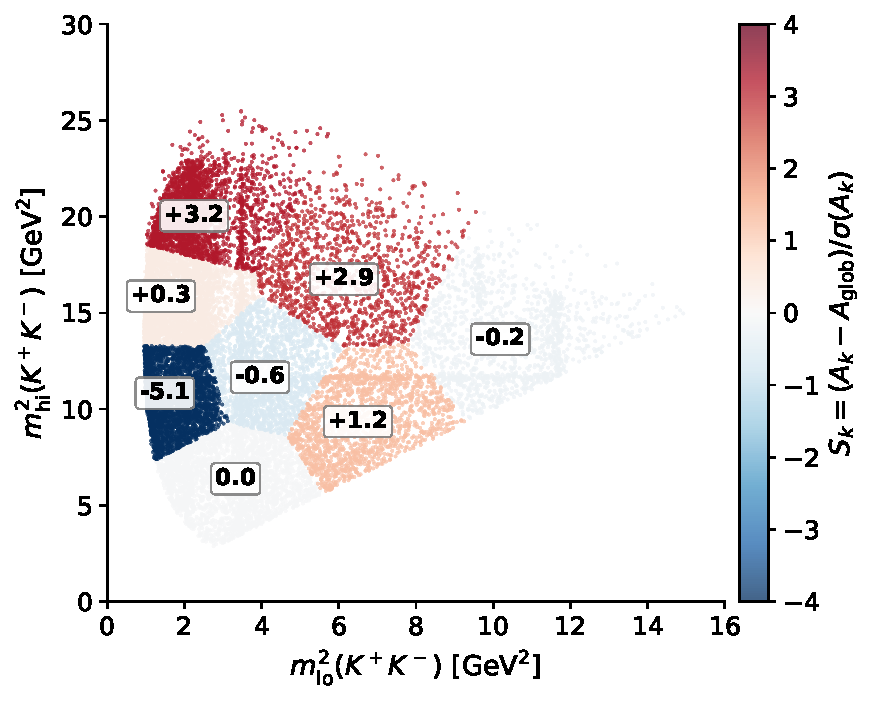
\includegraphics[width=\columnwidth]{figures/short_ml_kmeans.pdf}
\caption{$K$-means partition ($K=8$) of the Dalitz plane, all candidates of the fit window, same axes as Fig.~\ref{fig:bayes_dalitz}. Color and labels: local significance of each cluster with respect to the global asymmetry, $S_k=(A_k-A_{\mathrm{glob}})/\sigma(A_k)$, on the same scale as panel (c) of Fig.~\ref{fig:bayes_dalitz}.}
\label{fig:ml_kmeans}
\end{figure}

\begin{figure}[h]
\centering
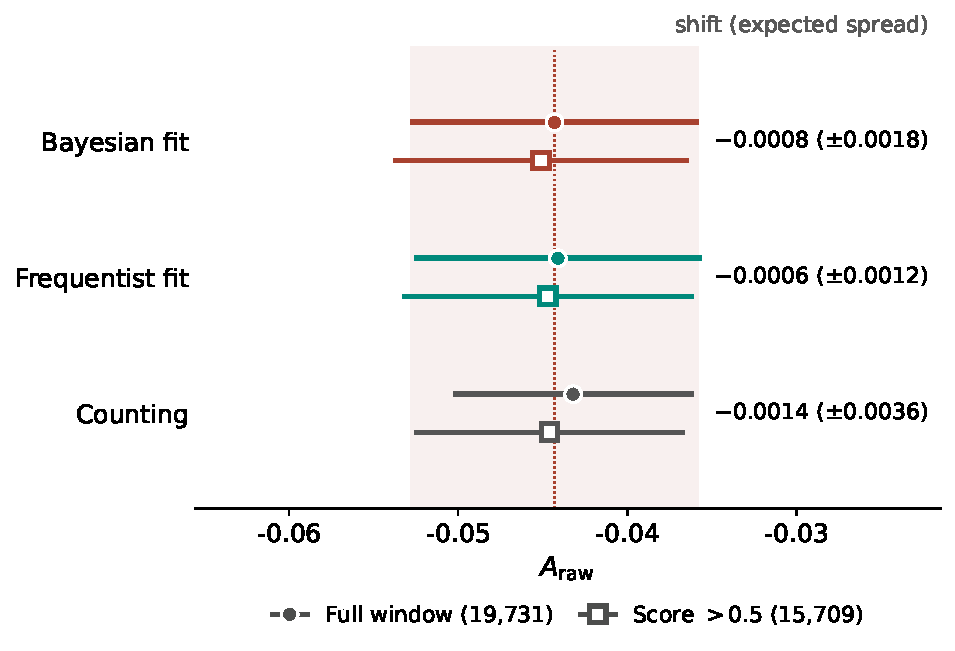
\includegraphics[width=\columnwidth]{figures/short_ml_three.pdf}
\caption{$\Araw$ from the Bayesian fit, the Frequentist fit and counting, for the full sample and the ML-selected ones, at a score cut of $0.5$ and at $0.73$, the maximum of the significance improvement.}
\label{fig:ml_three}
\end{figure}

